% Options for packages loaded elsewhere
% Options for packages loaded elsewhere
\PassOptionsToPackage{unicode}{hyperref}
\PassOptionsToPackage{hyphens}{url}
\PassOptionsToPackage{dvipsnames,svgnames,x11names}{xcolor}
%
\documentclass[
  letterpaper,
  DIV=11,
  numbers=noendperiod]{scrartcl}
\usepackage{xcolor}
\usepackage[top=30mm,left=30mm]{geometry}
\usepackage{amsmath,amssymb}
\setcounter{secnumdepth}{-\maxdimen} % remove section numbering
\usepackage{iftex}
\ifPDFTeX
  \usepackage[T1]{fontenc}
  \usepackage[utf8]{inputenc}
  \usepackage{textcomp} % provide euro and other symbols
\else % if luatex or xetex
  \usepackage{unicode-math} % this also loads fontspec
  \defaultfontfeatures{Scale=MatchLowercase}
  \defaultfontfeatures[\rmfamily]{Ligatures=TeX,Scale=1}
\fi
\usepackage{lmodern}
\ifPDFTeX\else
  % xetex/luatex font selection
\fi
% Use upquote if available, for straight quotes in verbatim environments
\IfFileExists{upquote.sty}{\usepackage{upquote}}{}
\IfFileExists{microtype.sty}{% use microtype if available
  \usepackage[]{microtype}
  \UseMicrotypeSet[protrusion]{basicmath} % disable protrusion for tt fonts
}{}
\makeatletter
\@ifundefined{KOMAClassName}{% if non-KOMA class
  \IfFileExists{parskip.sty}{%
    \usepackage{parskip}
  }{% else
    \setlength{\parindent}{0pt}
    \setlength{\parskip}{6pt plus 2pt minus 1pt}}
}{% if KOMA class
  \KOMAoptions{parskip=half}}
\makeatother
% Make \paragraph and \subparagraph free-standing
\makeatletter
\ifx\paragraph\undefined\else
  \let\oldparagraph\paragraph
  \renewcommand{\paragraph}{
    \@ifstar
      \xxxParagraphStar
      \xxxParagraphNoStar
  }
  \newcommand{\xxxParagraphStar}[1]{\oldparagraph*{#1}\mbox{}}
  \newcommand{\xxxParagraphNoStar}[1]{\oldparagraph{#1}\mbox{}}
\fi
\ifx\subparagraph\undefined\else
  \let\oldsubparagraph\subparagraph
  \renewcommand{\subparagraph}{
    \@ifstar
      \xxxSubParagraphStar
      \xxxSubParagraphNoStar
  }
  \newcommand{\xxxSubParagraphStar}[1]{\oldsubparagraph*{#1}\mbox{}}
  \newcommand{\xxxSubParagraphNoStar}[1]{\oldsubparagraph{#1}\mbox{}}
\fi
\makeatother


\usepackage{longtable,booktabs,array}
\newcounter{none} % for unnumbered tables
\usepackage{calc} % for calculating minipage widths
% Correct order of tables after \paragraph or \subparagraph
\usepackage{etoolbox}
\makeatletter
\patchcmd\longtable{\par}{\if@noskipsec\mbox{}\fi\par}{}{}
\makeatother
% Allow footnotes in longtable head/foot
\IfFileExists{footnotehyper.sty}{\usepackage{footnotehyper}}{\usepackage{footnote}}
\makesavenoteenv{longtable}
\usepackage{graphicx}
\makeatletter
\newsavebox\pandoc@box
\newcommand*\pandocbounded[1]{% scales image to fit in text height/width
  \sbox\pandoc@box{#1}%
  \Gscale@div\@tempa{\textheight}{\dimexpr\ht\pandoc@box+\dp\pandoc@box\relax}%
  \Gscale@div\@tempb{\linewidth}{\wd\pandoc@box}%
  \ifdim\@tempb\p@<\@tempa\p@\let\@tempa\@tempb\fi% select the smaller of both
  \ifdim\@tempa\p@<\p@\scalebox{\@tempa}{\usebox\pandoc@box}%
  \else\usebox{\pandoc@box}%
  \fi%
}
% Set default figure placement to htbp
\def\fps@figure{htbp}
\makeatother


% definitions for citeproc citations
\NewDocumentCommand\citeproctext{}{}
\NewDocumentCommand\citeproc{mm}{%
  \begingroup\def\citeproctext{#2}\cite{#1}\endgroup}
\makeatletter
 % allow citations to break across lines
 \let\@cite@ofmt\@firstofone
 % avoid brackets around text for \cite:
 \def\@biblabel#1{}
 \def\@cite#1#2{{#1\if@tempswa , #2\fi}}
\makeatother
\newlength{\cslhangindent}
\setlength{\cslhangindent}{1.5em}
\newlength{\csllabelwidth}
\setlength{\csllabelwidth}{3em}
\newenvironment{CSLReferences}[2] % #1 hanging-indent, #2 entry-spacing
 {\begin{list}{}{%
  \setlength{\itemindent}{0pt}
  \setlength{\leftmargin}{0pt}
  \setlength{\parsep}{0pt}
  % turn on hanging indent if param 1 is 1
  \ifodd #1
   \setlength{\leftmargin}{\cslhangindent}
   \setlength{\itemindent}{-1\cslhangindent}
  \fi
  % set entry spacing
  \setlength{\itemsep}{#2\baselineskip}}}
 {\end{list}}
\usepackage{calc}
\newcommand{\CSLBlock}[1]{\hfill\break\parbox[t]{\linewidth}{\strut\ignorespaces#1\strut}}
\newcommand{\CSLLeftMargin}[1]{\parbox[t]{\csllabelwidth}{\strut#1\strut}}
\newcommand{\CSLRightInline}[1]{\parbox[t]{\linewidth - \csllabelwidth}{\strut#1\strut}}
\newcommand{\CSLIndent}[1]{\hspace{\cslhangindent}#1}



\setlength{\emergencystretch}{3em} % prevent overfull lines

\providecommand{\tightlist}{%
  \setlength{\itemsep}{0pt}\setlength{\parskip}{0pt}}



 


\KOMAoption{captions}{tableheading}
\makeatletter
\@ifpackageloaded{tcolorbox}{}{\usepackage[skins,breakable]{tcolorbox}}
\@ifpackageloaded{fontawesome5}{}{\usepackage{fontawesome5}}
\definecolor{quarto-callout-color}{HTML}{909090}
\definecolor{quarto-callout-note-color}{HTML}{0758E5}
\definecolor{quarto-callout-important-color}{HTML}{CC1914}
\definecolor{quarto-callout-warning-color}{HTML}{EB9113}
\definecolor{quarto-callout-tip-color}{HTML}{00A047}
\definecolor{quarto-callout-caution-color}{HTML}{FC5300}
\definecolor{quarto-callout-color-frame}{HTML}{acacac}
\definecolor{quarto-callout-note-color-frame}{HTML}{4582ec}
\definecolor{quarto-callout-important-color-frame}{HTML}{d9534f}
\definecolor{quarto-callout-warning-color-frame}{HTML}{f0ad4e}
\definecolor{quarto-callout-tip-color-frame}{HTML}{02b875}
\definecolor{quarto-callout-caution-color-frame}{HTML}{fd7e14}
\makeatother
\makeatletter
\@ifpackageloaded{caption}{}{\usepackage{caption}}
\AtBeginDocument{%
\ifdefined\contentsname
  \renewcommand*\contentsname{Table of contents}
\else
  \newcommand\contentsname{Table of contents}
\fi
\ifdefined\listfigurename
  \renewcommand*\listfigurename{List of Figures}
\else
  \newcommand\listfigurename{List of Figures}
\fi
\ifdefined\listtablename
  \renewcommand*\listtablename{List of Tables}
\else
  \newcommand\listtablename{List of Tables}
\fi
\ifdefined\figurename
  \renewcommand*\figurename{Figure}
\else
  \newcommand\figurename{Figure}
\fi
\ifdefined\tablename
  \renewcommand*\tablename{Table}
\else
  \newcommand\tablename{Table}
\fi
}
\@ifpackageloaded{float}{}{\usepackage{float}}
\floatstyle{ruled}
\@ifundefined{c@chapter}{\newfloat{codelisting}{h}{lop}}{\newfloat{codelisting}{h}{lop}[chapter]}
\floatname{codelisting}{Listing}
\newcommand*\listoflistings{\listof{codelisting}{List of Listings}}
\makeatother
\makeatletter
\makeatother
\makeatletter
\@ifpackageloaded{caption}{}{\usepackage{caption}}
\@ifpackageloaded{subcaption}{}{\usepackage{subcaption}}
\makeatother
\usepackage{bookmark}
\IfFileExists{xurl.sty}{\usepackage{xurl}}{} % add URL line breaks if available
\urlstyle{same}
\hypersetup{
  pdftitle={Creating a positive learning environment},
  pdfauthor={Sarah von Grebmer zu Wolfsthurn},
  colorlinks=true,
  linkcolor={blue},
  filecolor={Maroon},
  citecolor={Blue},
  urlcolor={Blue},
  pdfcreator={LaTeX via pandoc}}


\title{Creating a positive learning environment}
\author{Sarah von Grebmer zu Wolfsthurn}
\date{21/08/2026}
\begin{document}
\maketitle


\subsection{Licence}\label{licence}

This current work by Sarah von Grebmer zu Wolfsthurn, Sara Lil Middleton
and Malika Ihle is licensed under a CC-BY-SA 4.0
\href{https://creativecommons.org/licenses/by-sa/4.0/deed.en}{Creative
Commons Attribution 4.0 International SA License}. It permits
unrestricted re-use, distribution, and reproduction in any medium,
provided the original work is properly cited. If you remix, transform,
or build upon the material, you must distribute your contributions under
the same license as the original.

\textbf{Presenter Notes}: The Creative Commons Attribution--ShareAlike
4.0 license, or CC BY-SA 4.0, allows others to copy, share, and adapt a
work in any medium, including for commercial purposes. These permissions
are broad and cannot be withdrawn as long as the license terms are
followed. The main requirement is attribution: users must give
appropriate credit to the original creator, provide a link to the
license, and clearly indicate whether any changes were made, without
implying endorsement by the original author. In addition, the ShareAlike
condition means that if someone modifies or builds upon the work, the
resulting material must be distributed under the same CC BY-SA 4.0
license, or a compatible one. Finally, users are not allowed to apply
legal or technical restrictions, such as DRM, that would prevent others
from exercising these same rights.

\begin{center}\rule{0.5\linewidth}{0.5pt}\end{center}

\subsection{Contribution statement}\label{contribution-statement}

\textbf{Creator}: Von Grebmer zu Wolfsthurn, Sarah
(\pandocbounded{
\includegraphics[keepaspectratio]{images/ORCID-iD_icon_16x16.png}}
\href{https://orcid.org/0000-0002-6413-3895}{0000-0002-6413-3895})

\textbf{Reviewer}: Middleton, Sara
(\pandocbounded{
\includegraphics[keepaspectratio]{images/ORCID-iD_icon_16x16.png}}\href{https://orcid.org/0000-0001-5307-8029}{0000-0001-5307-8029})

\textbf{Consultant}: Ihle, Malika
(\pandocbounded{
\includegraphics[keepaspectratio]{images/ORCID-iD_icon_16x16.png}}
\href{https://orcid.org/0000-0002-3242-5981}{0000-0002-3242-5981})

\textbf{Presenter Notes}: These are the \textbf{presenter notes}. You
will a script for the presenter for every slide. In presentation mode,
your audience will not be able to see these presenter notes, they are
only visible to the presenter.

\textbf{Instructor Notes}: There are also \textbf{instructor notes}. For
some slides, there will be pedagogical tips, suggestions for activites
and troubleshooting tips for issues your audience might run into. You
can find these notes underneath the presenter notes.

\textbf{Accessibility Tips}: Where applicable, this is a space to add
any tips you may have to facilitate the accessibility of your slides and
activities.

\begin{center}\rule{0.5\linewidth}{0.5pt}\end{center}

\subsection{Prerequisites - EDIT}\label{prerequisites---edit}

\begin{tcolorbox}[enhanced jigsaw, arc=.35mm, bottomrule=.15mm, bottomtitle=1mm, breakable, colback=white, colbacktitle=quarto-callout-important-color!10!white, colframe=quarto-callout-important-color-frame, coltitle=black, left=2mm, leftrule=.75mm, opacityback=0, opacitybacktitle=0.6, rightrule=.15mm, title=\textcolor{quarto-callout-important-color}{\faExclamation}\hspace{0.5em}{Important}, titlerule=0mm, toprule=.15mm, toptitle=1mm]

Before completing this session, please carefully read about the
prerequisites.

\end{tcolorbox}

{\def\LTcaptype{none} % do not increment counter
\begin{longtable}[]{@{}
  >{\raggedright\arraybackslash}p{(\linewidth - 4\tabcolsep) * \real{0.3333}}
  >{\raggedright\arraybackslash}p{(\linewidth - 4\tabcolsep) * \real{0.3333}}
  >{\raggedright\arraybackslash}p{(\linewidth - 4\tabcolsep) * \real{0.3333}}@{}}
\toprule\noalign{}
\begin{minipage}[b]{\linewidth}\raggedright
Prerequisite
\end{minipage} & \begin{minipage}[b]{\linewidth}\raggedright
Description
\end{minipage} & \begin{minipage}[b]{\linewidth}\raggedright
Link/Where to find it
\end{minipage} \\
\midrule\noalign{}
\endhead
\bottomrule\noalign{}
\endlastfoot
Basic familiarity with Open Science practices & Examples: R, Quarto,
Git, GitHub, preregistration, Open Access etc. &
\href{https://lmu-osc.github.io/train-the-trainer-student-track-OS/}{Click
here to get familiar with Open Science first} \\
Core didactic principles & A firm grasp on important didactic tools and
elements & \href{https://quarto.org}{Download Link} \\
Knowledge about designing teaching events & Tools and strategies to
create a learning experience to convey content and skills &
\href{https://quarto.org}{Download Link} \\
\end{longtable}
}

\textbf{Presenter Notes}: For this session, it is important that you
have previously thought about didactics and incorporating pedagogical
elements in your teaching. You should be familiar with the basics of
what learning means, the framework of constructivism, constructive
alignment and how to set and formulate learning objectives If you are
not yet familiar with these concepts, please see the previous session on
``Core didactic principles'' when teaching about Open Research or Open
Science.

\textbf{Instructor Notes}: These are the prerequisites for this session.
Before you get started on this session with your audience, you need to
ensure that the audience fulfills these criteria.

\begin{center}\rule{0.5\linewidth}{0.5pt}\end{center}

\subsection{Questions from the previous
session}\label{questions-from-the-previous-session}

What are your questions from the previous session?

\textbf{Presenter Notes}: What were your questions from the previous
session? \textbf{Instructor Notes}: Instead of asking ``Do you have any
questions'', work under the assumption that there are questions to show
your learners that it is normal to ask questions and to still be unsure
about specific elements of previous sessions. Instead, ask ``What are
your questions''.

\begin{center}\rule{0.5\linewidth}{0.5pt}\end{center}

\subsection{Key terms and definitions}\label{key-terms-and-definitions}

\begin{itemize}
\tightlist
\item
  \textbf{Learning environment}:
\item
  \textbf{Active listening}:
\item
  \textbf{Growth mindset}:
\item
  \textbf{Inclusive language}:
\end{itemize}

\textbf{Presenter Notes}: Here are some key concepts we will be
discussing throughout the session. Think for yourself what each one of
these concepts means to you at this points, or have an educated guess
based on your experience what the key term could mean. Then, discuss
with your partner. We will then briefly discuss the terms in the plenum.
At the end of the session, we will come back to these terms and you will
have formed new concepts relared to each of these terms.

\textbf{Instructor Notes}: Identify prior knowledge of learners at this
point and come back to possible misconceptions throughout the session.
Use the think-pair-share method. Allow for about 5 minutes for this
exercise.

\begin{center}\rule{0.5\linewidth}{0.5pt}\end{center}

\subsection{Key terms and
definitions}\label{key-terms-and-definitions-1}

\begin{itemize}
\tightlist
\item
  \textbf{Learning environment}: Comprises ``the psychological,
  cultural, and physical setting in which learning occurs and in which
  experiences and expectations are co-created among its participants''
  (Rusticus et al., 2023)
\item
  \textbf{Active listening}: ``The deliberate process of listening with
  attention and intention to understand another person's message, while
  showing that understanding through responses such as clarification,
  reflection, and feedback.''
  (\href{https://www.cmu.edu/student-affairs/civility/resources/active-listening.html}{Carnegie
  Mellon University})
\item
  \textbf{Growth mindset}: ``The ability to reframe perceived failures
  as opportunities to learn and grow'' (Dweck, 2006)
\item
  \textbf{Inclusive language}: Language that acknowledges the diversity
  of people, avoids stereotypes, discrimination and assumptions and
  supports equal opportunities
  (\href{https://www.un.org/en/gender-inclusive-language/}{United
  Nations})
\end{itemize}

\begin{center}\rule{0.5\linewidth}{0.5pt}\end{center}

\subsection{Covered in this session}\label{covered-in-this-session}

\begin{itemize}
\tightlist
\item
  What \emph{is} a positive \textbf{learning environment}?
\item
  \textbf{Behaviors} and \textbf{attitudes} towards your audience
\item
  Fostering a \textbf{growth mindset}
\item
  Establishing \textbf{norms for interactions}
\item
  Universal Design for Learning (UDL)
\item
  \textbf{Inclusive language} in your Open Research (OR) event
\item
  \textbf{Taking perspective} and being a \textbf{role model} in your OR
  event
\end{itemize}

\textbf{Presenter Notes}: This is a little roadmap to what we will be
discussing today. All of it falls under the framework of ``What is a
positive learning environment, what can I do to create one and what does
it mean for my Open Research event?

\begin{itemize}
\tightlist
\item
  What \emph{is} a positive learning environment?
\item
  Behaviors and attitudes towards your audience
\item
  Fostering a growth mindset
\item
  Establishing norms for interactions
\item
  Universal Design for Learning (UDL)
\item
  Inclusive language
\item
  Perspective-taking and being a role model
\end{itemize}

\begin{center}\rule{0.5\linewidth}{0.5pt}\end{center}

\subsection{Learning objectives}\label{learning-objectives}

At the end of this session, you will be able to:

\begin{itemize}
\tightlist
\item
  \textbf{Describe} the key features of a positive learning environment,
  including the roles of verbal strategies, body language, growth
  mindset, interaction norms, perspective-taking, role modelling and
  inclusive language
\item
  \textbf{Evaluate} how your behavior, language, and attitude influence
  learner motivation and engagement
\item
  \textbf{Analyze} challenges affecting the learning environment during
  an Open Research training event and \textbf{evaluate} strategies to
  address them in different teaching contexts
\end{itemize}

\textbf{Presenter Notes}: In this session, we will explore how to create
and maintain a positive learning environment in Open Research training.

By the end of the session, you will be able to identify key elements
that contribute to a supportive learning environment, reflect on how
your own communication and behavior influence learners, and recognize
challenges that may affect participation and engagement.

\begin{center}\rule{0.5\linewidth}{0.5pt}\end{center}

\subsection{Before we start: Survey
time!}\label{before-we-start-survey-time}

ADD QR code

\textbf{Presenter Notes}: Let us briefly look at where you are at.

\textbf{Instructor Notes}: - \textbf{Aim}: The pre-session survey serves
to examine learners' prior knowledge about the session's topic. - Use
free survey software such as particify to establish the following
questions (shown on separate slides).

\begin{center}\rule{0.5\linewidth}{0.5pt}\end{center}

\subsection{Before we start: Survey
time!}\label{before-we-start-survey-time-1}

\subsubsection{Question 1}

\textbf{What is your experience with actively creating a positive
learning environment for your learners in Open Open Research events?}

\begin{enumerate}
\def\labelenumi{\alph{enumi}.}
\item
  I have never organized an Open Research event, so this does not apply
\item
  I am not familiar with the concept of a positive learning environment
  yet
\item
  I am familiar with the concept of a positive learning environment, but
  have not actively taken any steps towards it yet
\item
  I am familiar with the concept of a positive learning environment and
  have actively taken steps towards it
\item
  Creating a positive learning environment for your learners is all I
  think about for my Open Research events
\end{enumerate}

\subsubsection{Question 2}

\textbf{What is your level of familiarity with Universal Design for
Learning (UDL)?}

\begin{enumerate}
\def\labelenumi{\alph{enumi}.}
\item
  I have not heard of it yet
\item
  I have heard of it but have never actively engaged with it.
\item
  I have a basic understanding and use it sometimes in my teaching and
  learner interactions.
\item
  I am very familiar and use it extensively in my teaching and learner
  interactions.
\end{enumerate}

\subsubsection{Question 3}

\textbf{Which of the following elements of creating a positive learning
environment do you feel most confident about in your teaching?}

\begin{enumerate}
\def\labelenumi{\alph{enumi}.}
\item
  Using verbal strategies
\item
  Using non-verbal strategies
\item
  Fostering a growth mindset
\item
  Establishing norms for interaction
\item
  Using inclusive language
\item
  None of the above
\end{enumerate}

\begin{center}\rule{0.5\linewidth}{0.5pt}\end{center}

\subsection{Discussion of survey
results}\label{discussion-of-survey-results}

What do we see in the results?

\textbf{Presenter Notes}: Let us have a look at these results.

\textbf{Instructor Notes}: Briefly examine the answers given to each
question interactively with the group. Use visuals from the survey to
highlight specific answers.

\textbf{Accessibility Tip}: Have people work in pairs if someone did not
bring their phone/does not have a phone. This survey also cannot be
completed in an asynchronous setting.

\begin{center}\rule{0.5\linewidth}{0.5pt}\end{center}

\subsection{The ``learning
environment''}\label{the-learning-environment}

\textbf{What does this mean to you?}

Add QR code.

\emph{Take 5 minutes to collect some concepts and thoughts that come to
mind with your neighbor.}

\textbf{Presenter Notes}: First question to you as the audience: What
does the term learning environment mean to you? What thoughts or
concepts come to mind? Take 5 minutes to collect some concepts and
thoughts that come to mind with your neighbor. Use the QR code.

\textbf{Instructor Notes}: Collect thoughts with an interactive tool,
such as a wordcloud or similar (e.g., with the software Particify).
Highlight terms that were said more often by your learners, and also
some that were mentioned only once.

\begin{center}\rule{0.5\linewidth}{0.5pt}\end{center}

\subsection{The ``learning
environment''}\label{the-learning-environment-1}

``The \textbf{learning environment} comprises the \textbf{psychological,
social, cultural, and physical setting} in which learning occurs and in
which experiences and expectations are co-created among its
participants.''

``{[}\ldots{]} is the setting and conditions {[}\ldots{]} which
\textbf{influences} learners \textbf{engagement} and \textbf{success}.''

See Rusticus et al. (2023). Adapted from
\url{https://www.oecd.org/en/topics/policy-issues/learning-environment.html}.

\textbf{Presenter Notes}: When we talk about the learning environment,
we mean much more than the physical classroom or the online platform. It
includes the psychological, social, cultural, and physical conditions in
which learning takes place.

These different aspects shape how people experience learning. For
example, whether learners feel respected, included, supported, and able
to participate can influence their engagement with the course.

The learning environment is also something that everyone helps create.
Learners, instructors, and others involved all contribute through their
interactions, expectations, and behaviors.

Research suggests that a positive learning environment can support
learner engagement and success. This is why it is useful to think about
not only what we teach, but also the conditions in which learning
happens.

\textbf{Instructor Notes}: Connect these ``official'' definitions with
what learners had already mentioned during the brainstorming slide.

\begin{center}\rule{0.5\linewidth}{0.5pt}\end{center}

\subsection{Why the learning environment
matters}\label{why-the-learning-environment-matters}

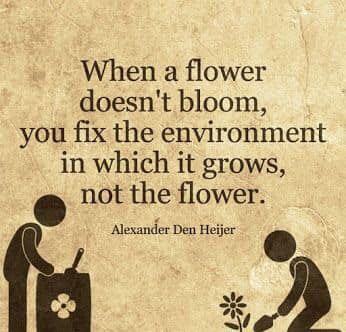
\includegraphics[width=1\linewidth,height=\textheight,keepaspectratio]{images/01-when-a-flower-doesnt-bloom.jpg}

- Influences \textbf{motivation} - Influences \textbf{performance} -
Influences \textbf{emotional well-being} - All linked to long-term
\textbf{knowledge retention} and increased \textbf{job competencies}

Rusticus et al. (2023)

\textbf{Presenter Notes}: Research shows that the learning environment
has a meaningful impact on learning outcomes. It can influence learners'
motivation to engage with a topic, seminar or course and their overall
performance.

The learning environment also affects emotional well-being. When
learners feel supported, respected, and psychologically safe, they are
generally better able to participate and learn.

Its impact can extend beyond the event or course itself. Positive
learning environments are associated with better long-term knowledge
retention and the development of competencies that learners can apply in
their professional roles.

In brief: it matters where and how you teach your learners, perhaps more
than you might think.

\begin{center}\rule{0.5\linewidth}{0.5pt}\end{center}

\subsection{Your turn! 5 minutes}\label{your-turn-5-minutes}

Activity: \textbf{What is a \emph{positive} learning environment?}
\emph{Write a few bullet points on what this means to you. Save this as
part of your developing teaching philosophy for future reference.}

\textbf{Presenter Notes}: Time for an activity! What is a positive
learning environment to you? What elements are in there? Write a few
bullet points on your thoughts and what you connect with this concept.
Save this as part of your developing teaching philosophy for future
reference in the workbook. Keep this in mind as we go along.

\textbf{Instructor Notes}: Plan about 5 minutes for this activity. Some
possible elements of a positive learning environment, see for example
three dimensions of Rusticus et al., 2023 from a learners perspective:
personal development (active learning in class, practical applications
of their learning, visuals, realistic expectations); relationships
(faculty support, peer interaction, group work); and institutional
setting (physical structure, expectations and culture of environment,
community, smaller class sizes).

\begin{center}\rule{0.5\linewidth}{0.5pt}\end{center}

\section{\texorpdfstring{What \emph{you} can do to create a positive
learning
environment?}{What you can do to create a positive learning environment?}}\label{what-you-can-do-to-create-a-positive-learning-environment}

\textbf{Presenter Notes}: In this next section, we will discuss
different methods and tools you can use to create a positive learning
environment. Note that for now, we will stay a little more general, but
throughout the following slides I want you to also think about how these
methods and tools could be implemented in an Open Research training
event where you are teaching about an Open Science topic.

\begin{center}\rule{0.5\linewidth}{0.5pt}\end{center}

\begin{center}\rule{0.5\linewidth}{0.5pt}\end{center}

\subsection{Verbal strategies}\label{verbal-strategies}

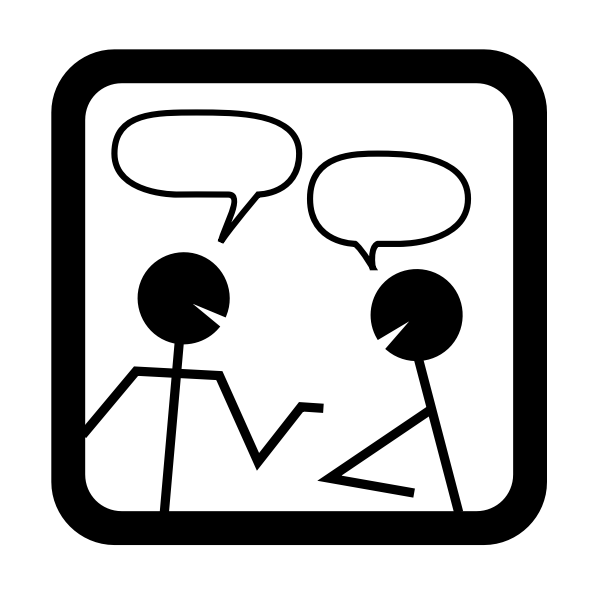
\includegraphics[width=0.7\linewidth,height=\textheight,keepaspectratio]{images/08-small-talk.png}

\begin{itemize}
\tightlist
\item
  \textbf{Small-talk} (yes, it is important)
\item
  Call learners by their \textbf{name}
\item
  \textbf{Validate} and show appreciation
\item
  Accept \textbf{silences}
\item
  Practice \textbf{active listening}
\end{itemize}

\begin{tcolorbox}[enhanced jigsaw, arc=.35mm, bottomrule=.15mm, bottomtitle=1mm, breakable, colback=white, colbacktitle=quarto-callout-note-color!10!white, colframe=quarto-callout-note-color-frame, coltitle=black, left=2mm, leftrule=.75mm, opacityback=0, opacitybacktitle=0.6, rightrule=.15mm, title=\textcolor{quarto-callout-note-color}{\faInfo}\hspace{0.5em}{Note}, titlerule=0mm, toprule=.15mm, toptitle=1mm]

Consider potential \textbf{language barriers} or \textbf{cultural
differences} in verbal communication, e.g., technical terms, high
vs.~low context cultures, feedback styles.

\end{tcolorbox}

Chat dialogue icon: OpenClipart / FreeSVG.org --- CC0 Public Domain.

\textbf{Presenter Notes}: Small, intentional actions can help create a
positive learning environment.

Starting with a little small talk before the event can help build
rapport and make learners feel more comfortable participating.

Using learners' names acknowledges them as individuals and can help
foster a sense of belonging.

Validating contributions and expressing appreciation encourages
participation, even when responses are incomplete or lead to further
discussion.

It is also helpful to be comfortable with silence. Giving learners time
to think can lead to more thoughtful responses and allows different
communication styles to be accommodated.

Finally, practicing active listening, a very valuable skill that is also
quite effective outside the teaching context.

\begin{center}\rule{0.5\linewidth}{0.5pt}\end{center}

\subsection{The skill of active
listening}\label{the-skill-of-active-listening}

``\,``\ldots{}\textbf{listening with attention and intention} to
understand another person's message, while \textbf{showing} that
\textbf{understanding} through responses such as clarification,
reflection, and feedback.''


\includegraphics[width=1\linewidth,height=\textheight,keepaspectratio]{images/02-active-listening.jpg}

\begin{itemize}
\tightlist
\item
  \textbf{Paraphrase} what audience members express
\item
  \textbf{Make} explicit \textbf{connections} between statements
\item
  \textbf{Refrain} from premature \textbf{judgment}
\item
  Ask for \textbf{clarification}
\item
  \textbf{Listen fully} before responding
\end{itemize}

Source:
\href{https://executive.berkeley.edu/thought-leadership/blog/art-active-listening}{UC
Berkely ExceEd Program}

\textbf{Presenter Notes}: Active listening is a skill that helps
learners feel heard and supports meaningful discussion.

Paraphrasing what someone has said helps confirm your understanding and
shows that you are listening carefully.

Making connections between different contributions can help learners see
relationships between ideas and build on each other's thinking.

Avoid rushing to evaluate or judge responses. Giving ideas space to
develop can encourage more open participation.

When something is unclear, ask for clarification rather than making
assumptions. This helps ensure shared understanding.

Finally, listen fully before responding. Allowing learners to finish
their thoughts demonstrates respect and leads to more thoughtful
conversations.

\textbf{Instructor Notes}: Highlight active listening as a transferrable
skill.

\begin{center}\rule{0.5\linewidth}{0.5pt}\end{center}

\subsection{Body language}\label{body-language}

\begin{itemize}
\tightlist
\item
  Maintain \textbf{eye contact} with learners
\item
  Use your \textbf{body for communication} \emph{(shake head, use
  hands)}
\end{itemize}

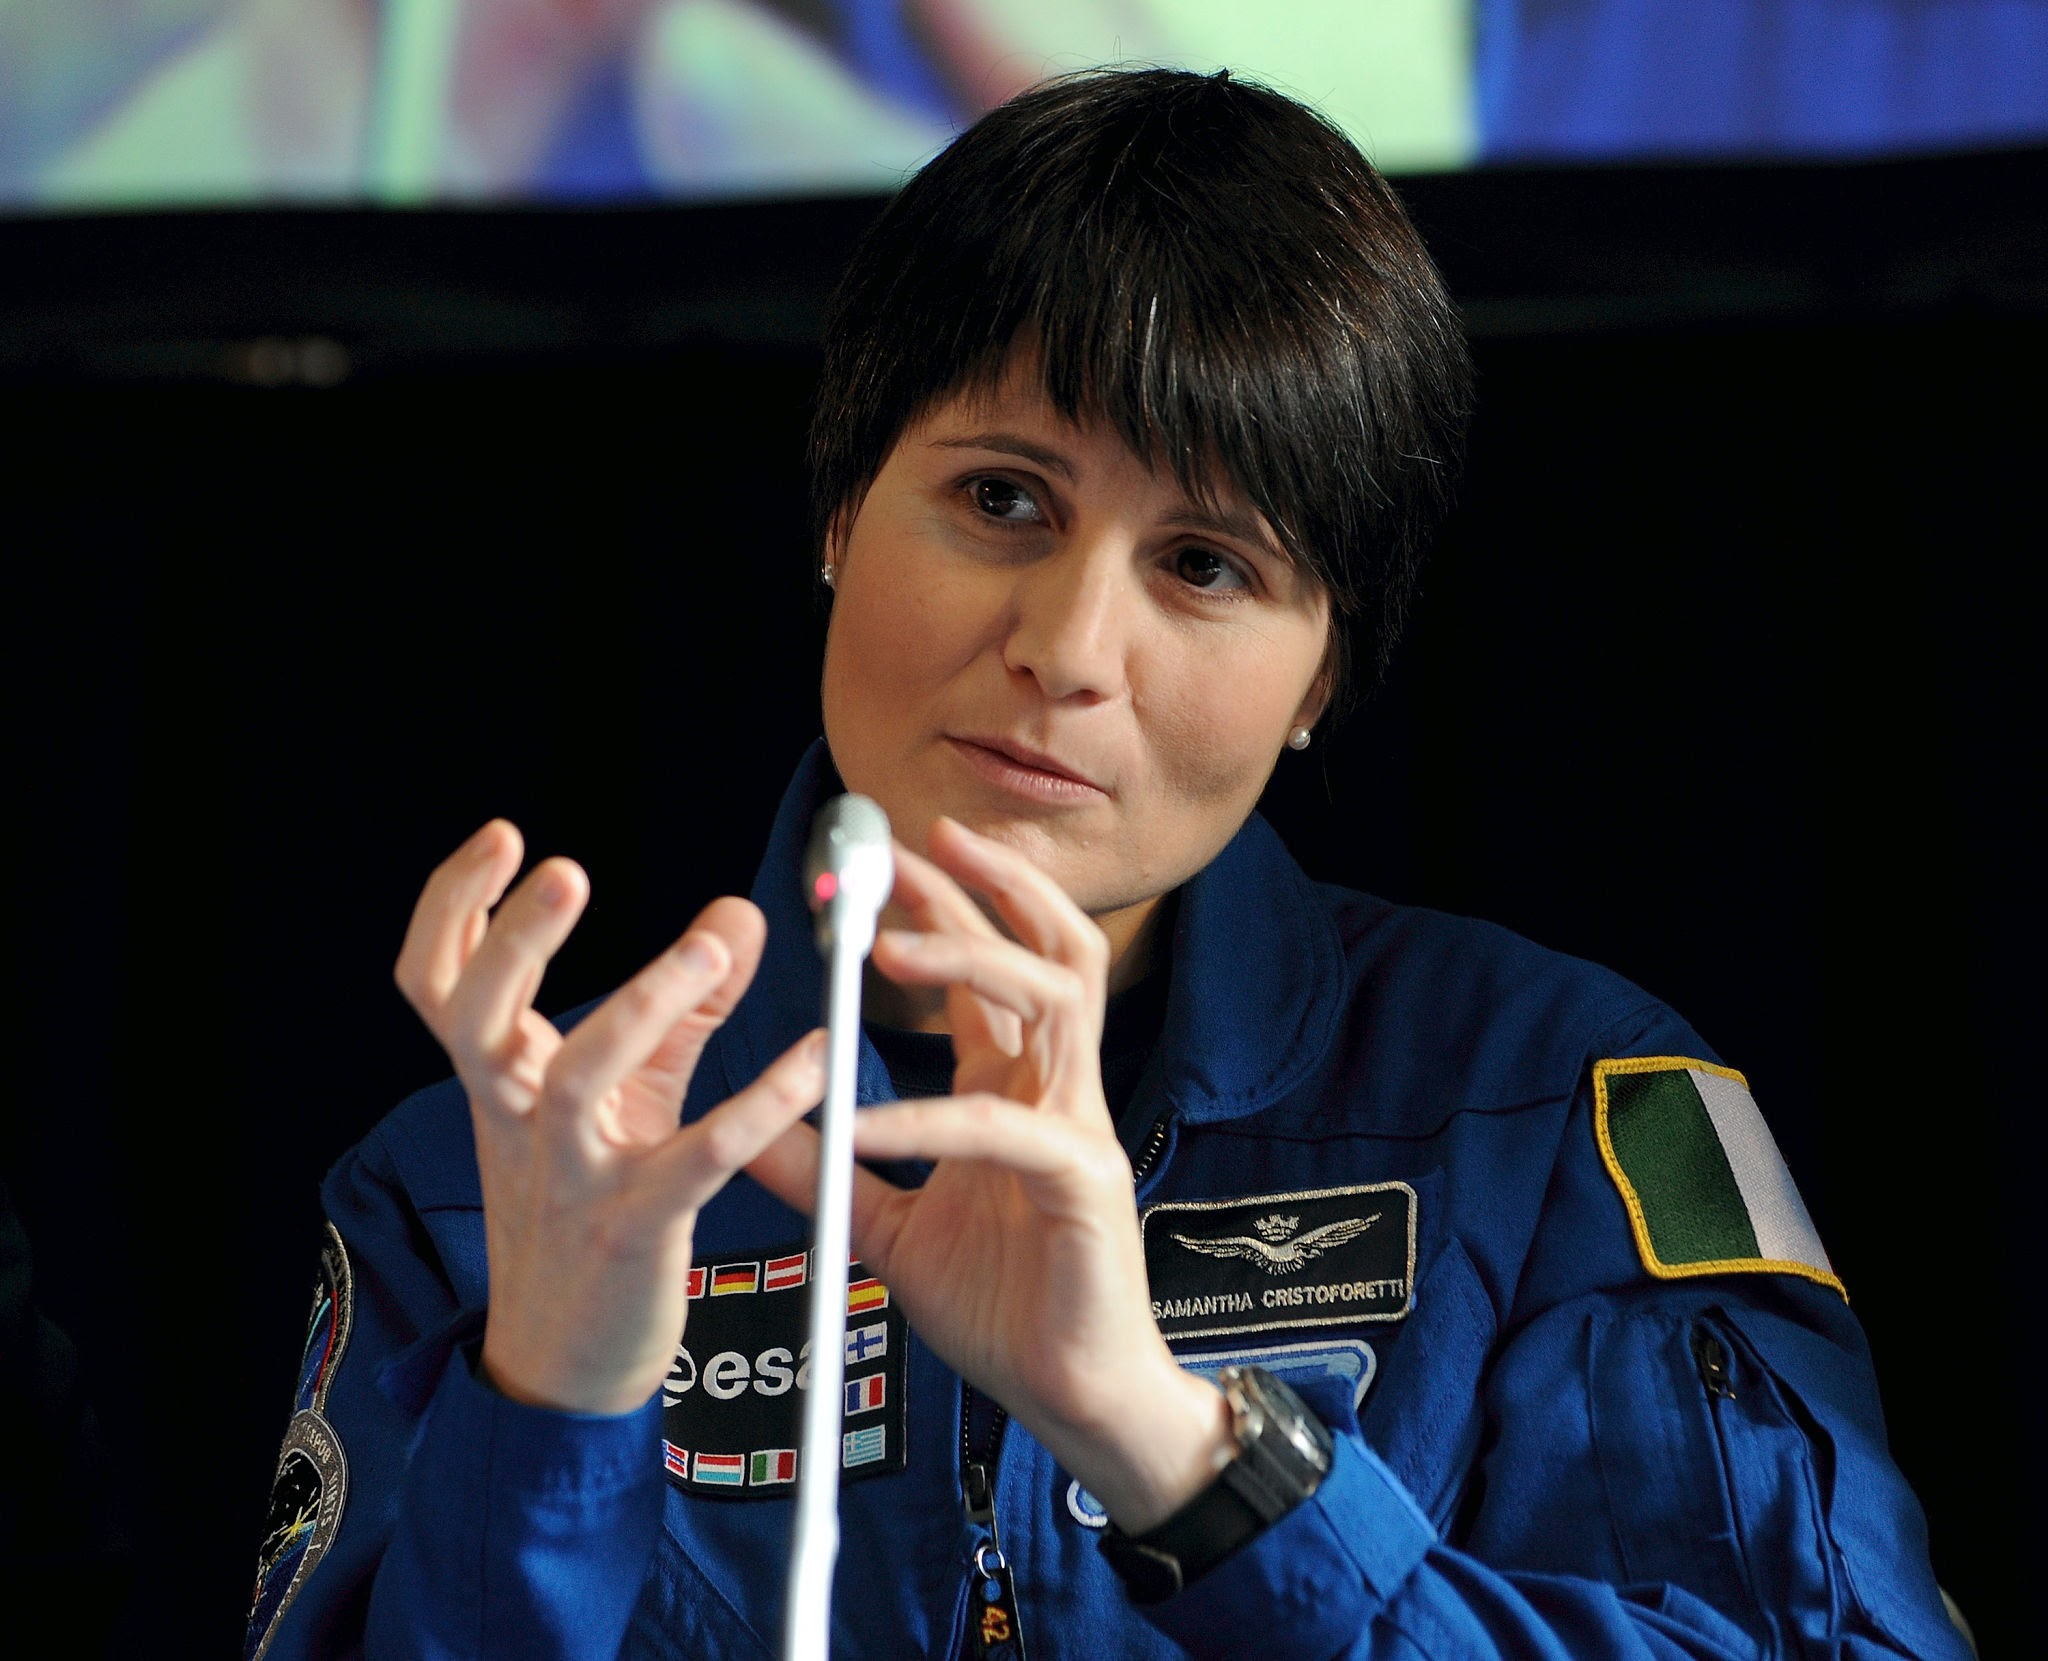
\includegraphics[width=0.8\linewidth,height=\textheight,keepaspectratio]{images/04-gesticulating.jpeg}

Astronaut Samantha Cristoforetti. Milan, Italy. Photo by Pier Marco
Tacca/Getty Images.

\begin{tcolorbox}[enhanced jigsaw, arc=.35mm, bottomrule=.15mm, bottomtitle=1mm, breakable, colback=white, colbacktitle=quarto-callout-note-color!10!white, colframe=quarto-callout-note-color-frame, coltitle=black, left=2mm, leftrule=.75mm, opacityback=0, opacitybacktitle=0.6, rightrule=.15mm, title=\textcolor{quarto-callout-note-color}{\faInfo}\hspace{0.5em}{Note}, titlerule=0mm, toprule=.15mm, toptitle=1mm]

Consider \textbf{cultural differences in body language}, e.g.,
perception of eye contact and body gestures.

\end{tcolorbox}

\textbf{Presenter Notes}: Body language can reinforce verbal
communication and help create a welcoming learning environment.

Maintaining appropriate eye contact can show that you are attentive and
engaged. At the same time, it's helpful to be mindful that comfort with
eye contact varies across individuals and cultures.

The meaning and interpretation of eye contact, gestures, and personal
space can vary, so being aware of these differences can help support
respectful and inclusive communication. For example, in many Western
cultures like Germany, Candada etc. direct eye contact is a sign of
confidence and engagement, whereas in other cultures it could be
considered confrontational in parts of Japan and South Korea

\begin{center}\rule{0.5\linewidth}{0.5pt}\end{center}

\subsection{Your turn: 7 minutes}\label{your-turn-7-minutes}

Activity: \textbf{Practice your active listening skills and observe your
body language while your peer is answering one of the questions below.}

\begin{itemize}
\item
  How did you first hear about Open Research practices or first become
  involved in them?
\item
  What does Open Research mean to you and your research work?
\item
  Do you already have an Open Research topic in mind you would like to
  teach about? What would it be and why?
\end{itemize}

Instructions: Groups of three, one learner, one instructor practicing
the active listening, one observer. Learner gives answer to question to
the instructor (approx. 2 mins). In the debriefing, discuss observations
and experiences with verbal and non-verbal communication.

\textbf{Presenter Notes}: Form groups of three, one is the learner, one
the instructor practicing the active listening, one the observer. The
learner picks one of the questions, then tells the instructor about
their thoughts on the question for approx. 2 minutes. The observer
focuses on body language and verbal communication. At the end of the two
minutes, discuss as the group. The learner goes first, and describes
their experience with the body language and verbal strategies of the
instructor. The observer shares their insights, and the instructor
shares how the exercise was for them.

\textbf{Instructor Notes}: Leave about 5 - 7 minutes for this exercise.

\begin{center}\rule{0.5\linewidth}{0.5pt}\end{center}

\subsection{Attitudes towards your audience:
methods}\label{attitudes-towards-your-audience-methods}

\begin{itemize}
\tightlist
\item
  Motivate audience to get involved as \textbf{early as possible}
\item
  Have \textbf{introductory activities}
\item
  Use different \textbf{visualization methods} to encourage
  \textbf{different ways of participation} \emph{(e.g., through
  speaking, chat, collaborative documents, whiteboards, anonymous
  questions\ldots)}
\item
  \textbf{Adapt} to your audience: pace, examples, level of difficulty
  \ldots{}
\end{itemize}


\includegraphics[width=0.7\linewidth,height=\textheight,keepaspectratio]{images/05-introduce-yourself.png}

\begin{tcolorbox}[enhanced jigsaw, arc=.35mm, bottomrule=.15mm, bottomtitle=1mm, breakable, colback=white, colbacktitle=quarto-callout-note-color!10!white, colframe=quarto-callout-note-color-frame, coltitle=black, left=2mm, leftrule=.75mm, opacityback=0, opacitybacktitle=0.6, rightrule=.15mm, title=\textcolor{quarto-callout-note-color}{\faInfo}\hspace{0.5em}{Note}, titlerule=0mm, toprule=.15mm, toptitle=1mm]

Consider \textbf{neurodiversity} when \textbf{designing engagement
activities and visualizations}: color choices, sensory processing,
mental imagery\ldots{}

\end{tcolorbox}

© 2018 Cristina Simmons

\textbf{Presenter Notes}: Besides verbal strategies and using your body
language, you can also create a positive learning environment through
different teaching methods. For example, introductory activities can
help learners get to know the topic, the instructor, and each other.
They can also create an opportunity for everyone to become involved
early on.

Encouraging participation at the start of a session can help establish
an environment where learners feel comfortable contributing and sharing
ideas.

Using different visualization methods and tools can support different
ways of engaging with information and can make learning more accessible.
With this, you can encourage different ways of participation
\emph{(e.g., through speaking, chat, collaborative documents,
whiteboards, anonymous questions\ldots)}

Finally, adapting to your audience means being responsive to their
needs, experiences, backgrounds, and level of understanding. This may
involve adjusting examples, explanations, pacing, or activities to
support effective learning.

\emph{Note}: When designing activities and visual materials, consider
that learners process information in different ways. Use clear visuals,
thoughtful color choices, and varied ways of engaging with content to
support different sensory and cognitive needs. For example, avoid
relying only on color to communicate meaning, consider sensory load in
activities, and provide enough structure for learners to process
information in their own way.

\textbf{Instructor Notes}: Refer back to what was collected in previous
exercises.

\begin{center}\rule{0.5\linewidth}{0.5pt}\end{center}

\subsection{Your turn! 6 minutes}\label{your-turn-6-minutes}

Activity:

\textbf{Collect introductory activities that you use in your teaching on
Open Research or saw in other Open Research training you attended and
describe what effect they had on you or the learners}.

\emph{Instructions: Write down some thoughts for yourself for 2 minutes,
then discuss with your neighbor for 2 minutes, then we will discuss in
the big group for 2 minutes.}

\textbf{Presenter Notes}: With these examples for methods in mind,
collect some introductory activities that you use in your teaching on
Open Research or have seen in other Open Research teaching events you
attended

\textbf{Instructor Notes}: Allow approx. 6 minutes for this exercise,
apply think-pair-share, two minutes each. Discuss as a group in the
``share'' phase.

\begin{center}\rule{0.5\linewidth}{0.5pt}\end{center}

\subsection{Fostering a growth
mindset}\label{fostering-a-growth-mindset}

\textbf{Growth mindset} = ``the ability to reframe perceived failures as
opportunities to learn and grow'' (Dweck, 2006)


\includegraphics[width=0.8\linewidth,height=\textheight,keepaspectratio]{images/12_growth_mindset.png}

\begin{itemize}
\tightlist
\item
  Positive \textbf{error framing}
\item
  Praise \textbf{effort and improvement}, not performance or ability
\item
  Provide opportunities for \textbf{self-assessment}
\item
  Present \textbf{multiple} possible \textbf{approaches}
\item
  Help your learners set \textbf{realistic expectations}
\end{itemize}

Adapted from Laura Carter: \url{https://zenodo.org/records/18905547}
\url{https://icons8.com/icons}

\textbf{Presenter Notes}: The idea of a growth mindset is that abilities
are not simply fixed, but can develop through learning, effort, and
effective strategies. The aim is therefore not to avoid errors or
failure, but to treat them as useful information for learning and
improvement.

In practice, this means framing errors constructively and giving
feedback that focuses on the learning process. Rather than praising
ability or intelligence, we can acknowledge meaningful effort, effective
strategies, and improvement. Importantly, effort alone is not enough:
when a strategy is not working, learners should be encouraged to try a
different approach or seek additional support.

Self-assessment can help learners reflect on what they understand, where
difficulties remain, and what they might try next. Providing several
possible approaches also makes clear that there is often more than one
way to solve a problem.

Finally, realistic expectations are important. A growth mindset does not
mean assuming that everyone can achieve anything immediately. It means
recognizing that progress is possible while being realistic about the
time, practice, strategies, and support that learning may require.

\begin{center}\rule{0.5\linewidth}{0.5pt}\end{center}

\subsection{Establish norms for
interaction}\label{establish-norms-for-interaction}

\textbf{Question: Which learning interactions will be common in your
event/course?} (\emph{e.g., large group discussions, work in pairs..})

\begin{itemize}
\tightlist
\item
  Based on this: \textbf{establish rules for interaction} (or a
  \emph{Code of }Conduct)
\item
  \textbf{Examples}:

  \begin{itemize}
  \tightlist
  \item
    Take group work \textbf{seriously}
  \item
    \textbf{Listen} respectfully, do not interrupt
  \item
    \textbf{Respect} different perspectives and experiences with Open
    Research, critique ideas, not people
  \item
    \textbf{Use inclusive language} and try to avoid assumptions about
    others
  \item
    \ldots{}
  \end{itemize}
\end{itemize}


\includegraphics[width=0.5\linewidth,height=\textheight,keepaspectratio]{images/11_code-of-conduct.png}

\url{https://crlt.umich.edu/examples-discussion-guidelines}
\url{https://zenodo.org/records/18905547}

\textbf{Presenter Notes}: Next, we want to discuss norms for
interacting. First, I need to think about what kind of interactions I am
expecting in my class. More group work, more discussions, interactive
things etc. Based on this, instructors could formulate a code of
conduct.

Examples:

\begin{itemize}
\tightlist
\item
  Take pair work or small group work seriously. Remember that your
  peers' learning is partly dependent upon your engagement.
\item
  Listen respectfully. Don't interrupt, turn to technology, or engage in
  private conversations while others are speaking. Use attentive,
  courteous body language. Comments that you make (whether asking for
  clarification, sharing critiques, or expanding on a point) should
  reflect that you have paid attention to the previous speakers'
  comments.
\item
  Respect different perspectives and experiences. Open Research involves
  different disciplines, communities, and research traditions, as well
  as different views on ``how research is done''.
\item
  Using inclusive language means choosing words and behaviors that
  recognize and respect the diversity of learners and avoid assumptions
  about people's identities, experiences, or abilities. Example
  non-inclusive language: ``you guys'', ``everyone knows that''
\end{itemize}

\begin{center}\rule{0.5\linewidth}{0.5pt}\end{center}

\subsection{Universal design for
learning}\label{universal-design-for-learning}

\begin{itemize}
\tightlist
\item
  Framework by \href{https://www.cast.org/}{CAST} to \textbf{improve and
  optimize teaching and learning} for \textbf{all people} based on
  scientific insights in how humans learn
\item
  Addresses \textbf{diversity in learning} in three categories:

  \begin{itemize}
  \tightlist
  \item
    \emph{Engagement} (the \textbf{why} of learning)
  \item
    \emph{Representation} (the \textbf{what} of learning)
  \item
    \emph{Action \& Expression} (the \textbf{how} of learning)
  \end{itemize}
\end{itemize}

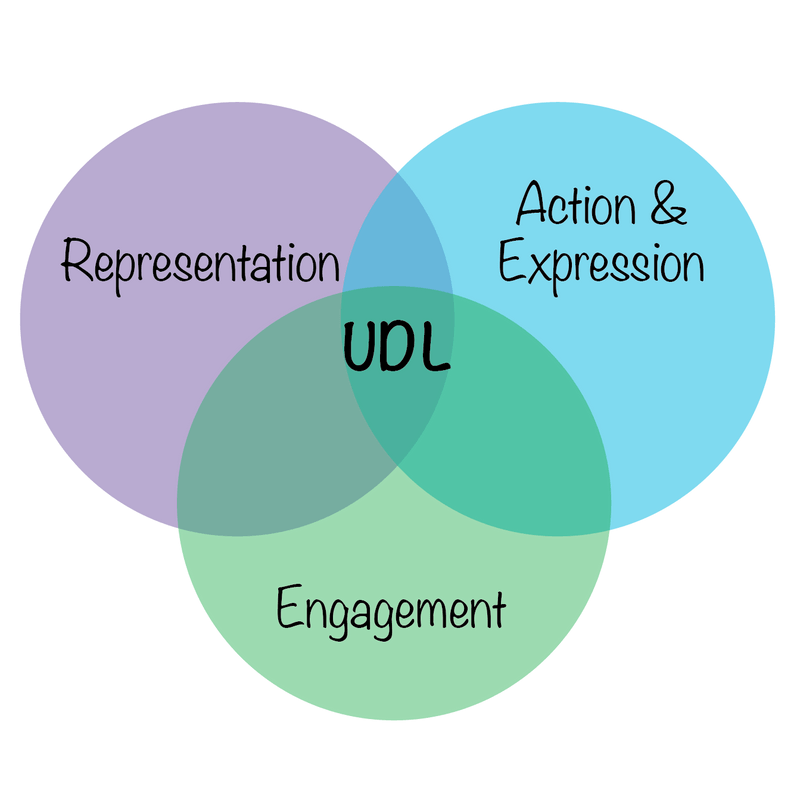
\includegraphics[width=1\linewidth,height=\textheight,keepaspectratio]{images/07-udl-summary.png}

\url{https://www.carleton.edu/its/blog/how-you-can-implement-universal-design-for-learning-udl-in-small-steps/}

\textbf{Presenter Notes}: Universal Design for Learning, or UDL, is a
framework developed by CAST that aims to improve and optimize teaching
and learning by considering the diversity of learners from the beginning
of the design process.

Rather than creating one approach and adapting it later for individual
needs, UDL encourages educators to provide flexible ways for learners to
engage with content, access information, and demonstrate their learning.

The framework is based on research about how people learn and focuses on
three key areas.

Engagement refers to the why of learning---how we motivate learners,
support their interests, and encourage active participation.

Representation refers to the what of learning---how information is
presented and whether learners have different ways to access and
understand content.

Action and Expression refers to the how of learning---how learners can
demonstrate their knowledge and skills through different methods.

We will not go into more detail here, but know that this is a framework
that can help you design your events and the content for a wider range
of learners.

\textbf{Instructor Notes}: Make an explicit link between norms of
interaction and UDL for a recognition effect, Provide a brief overview
about UDL and then refer to the resources.

\begin{center}\rule{0.5\linewidth}{0.5pt}\end{center}

\subsection{Expression: Inclusive
language}\label{expression-inclusive-language}

\textbf{= language} that acknowledges the \textbf{diversity of people},
\textbf{avoids} stereotypes, \textbf{discrimination} and assumptions and
supports \textbf{equal} opportunities (\emph{United Nations})


\includegraphics[width=0.8\linewidth,height=\textheight,keepaspectratio]{images/10_multicultural_audience.png}

\url{https://www.un.org/en/gender-inclusive-language/}
\url{https://icons8.com/icons}

\textbf{Presenter Notes}: Inclusive language is about choosing words and
communication styles that recognize and respect the diversity of people.

It means avoiding stereotypes, discrimination, and assumptions about
learners' identities, backgrounds, abilities, experiences, or knowledge.

In a learning environment, inclusive language helps create a sense of
belonging and supports equal opportunities for everyone to participate
and contribute. As instructors, we can choose the language we use during
our teaching.

\begin{center}\rule{0.5\linewidth}{0.5pt}\end{center}

\section{So.. what about creating a positive learning environment in
your Open Research
event?}\label{so..-what-about-creating-a-positive-learning-environment-in-your-open-research-event}

\textbf{Presenter Notes}: So\ldots{} what about creating a positive
learning environment when teaching Open Research? What could a positive
learning environment mean in that context? Where is the overlap?

\begin{center}\rule{0.5\linewidth}{0.5pt}\end{center}

\subsection{Language in your Open Research
event}\label{language-in-your-open-research-event}

\begin{itemize}
\item
  Use respectful and \textbf{person-centered language}

  \begin{itemize}
  \tightlist
  \item
    ``\textbf{Everyone}'', ``\textbf{all}'' etc. instead of ``\emph{You
    guys}''
  \end{itemize}
\item
  \textbf{Explain technical Open Research terms}, do not assume prior
  knowledge
\item
  \textbf{Use examples} from \textbf{different} research fields, not
  just one domain
\item
  Provide \textbf{multiple approaches} for a problem

  \begin{itemize}
  \tightlist
  \item
    ``\textbf{One approach is..}'' instead of ``\emph{Of course you
    would do it this way!}''
  \end{itemize}
\item
  \textbf{Avoid idioms, slang}, or culture-specific jokes

  \begin{itemize}
  \tightlist
  \item
    ``\textbf{Share your research output across different trusted
    platforms.}'' instead of ``\emph{Don't put all eggs into one
    basket!}''
  \end{itemize}
\end{itemize}

Phan et al. (2025)

\textbf{Presenter Notes}: Language in your Open Research event is of
highest importance. As we have seen, language is a massive part of the
learning environment and therefore of the learning experience and
process for your learners. It influences how learners feel, but also how
learners engage and participate. Here are some ideas for language in
your Open Research event:

\begin{itemize}
\item
  First, use respectful and person-centred language that recognizes
  participants as individuals and avoids reducing people to a single
  characteristic. Small changes, such as using ``everyone'' instead of
  ``you guys,'' can make communication more inclusive. At the same time,
  be mindful and respect people's preferences, normalize asking how to
  correctly pronounce someones name and be open to updating your
  language, for example pronouns).
\item
  Avoid assuming that participants share the same level of knowledge or
  experience. Explain technical Open Research concepts clearly and
  create opportunities for learners from different backgrounds to
  engage.
\item
  When presenting examples, include perspectives from different research
  fields to show that Open Research practices can apply across
  disciplines.
\item
  It is also important to acknowledge that there may be multiple valid
  ways to approach a challenge. Using language such as ``one approach
  is\ldots'' encourages exploration rather than suggesting there is only
  one correct solution.
\item
  Finally, avoid idioms, slang, or culture-specific references that may
  not be understood by everyone. Clear and accessible language helps
  ensure that all participants can fully engage with the content.
\end{itemize}

\textbf{Instructor Notes}: Cocnrete examples connected to Open Research:

\begin{itemize}
\item
  \emph{Less inclusive}: Everyone should already have Git installed. If
  not, you're behind.
\item
  \emph{More inclusive}: We will use Git during this session. If you
  have not installed it yet or run into issues, we will provide support
  to get everyone on the same page.
\end{itemize}

\begin{center}\rule{0.5\linewidth}{0.5pt}\end{center}

\subsection{Taking perspectives in your Open Research
event}\label{taking-perspectives-in-your-open-research-event}

\textbf{Do not assume.} Recognize that learners come to Open Research
from different:

\begin{itemize}
\tightlist
\item
  perspectives
\item
  disciplines
\item
  institutions
\item
  resources
\item
  access to (research) infrastructure
\item
  \ldots{}
\end{itemize}

\textbf{Presenter Notes}: It is very important to keep in mind that
Learners come to Open Research with different backgrounds and
experiences:

\begin{itemize}
\tightlist
\item
  \emph{Perspectives}: People may have different views on Open Research
  For example, one researcher may see preprints as a way to share
  findings quickly, while another may have concerns about sharing work
  before peer review.
\item
  \emph{Disciplines}: Open practices vary across fields. For example,
  open data sharing may be common in astronomy, while researchers in
  clinical studies may need to consider participant privacy and consent.
\item
  \emph{Institutions}: Researchers may have different levels of
  institutional support. For example, one university may offer Open
  Access funding and training, while another may provide fewer
  resources.
\item
  \emph{Resources}: Time, funding, and support can influence
  participation. For example, a large research centre may have dedicated
  data managers, while an independent researcher may manage these tasks
  alone.
\item
  \emph{Access to infrastructure}: Researchers may have different access
  to tools and platforms. For example, some may use institutional
  repositories, while others rely on public tools to share their work.
\end{itemize}

\begin{center}\rule{0.5\linewidth}{0.5pt}\end{center}

\subsection{Be a role model in your Open Research
event}\label{be-a-role-model-in-your-open-research-event}

\begin{itemize}
\tightlist
\item
  \textbf{Add anecdotes} about your own experiences with Open Research
  tools: ``\emph{To get this to work, I had to\ldots{}}''
\item
  \textbf{Show} your learners your \textbf{workflow}, e.g., your GitHub
  repository or folder structure
\item
  \textbf{Share mistakes} or uncertainties you encountered in your own
  workflow: ``\emph{I got my R plot wrong at first because..}''
\end{itemize}

\textbf{Presenter Notes}: One very powerful strategy to contribute to a
positive learning environment in Open Research is to be a role model.
For example:

\begin{itemize}
\tightlist
\item
  Add anecdotes: Briefly share examples from your own use of Open
  Science tools, including what worked well and what you learned along
  the way.
\item
  Show your workflows: Demonstrating your own GitHub repository, file
  organization, or documentation practices can help learners see how
  Open Research is applied in practice.
\item
  Share uncertainties and limitations: Being open about challenges in
  your workflow shows that Open Research is an ongoing process and
  encourages learners to reflect on their own practices.
\end{itemize}

\textbf{Instructor Notes}: Refer back to positive error framing when
discussing uncertainties and challenges in your Open Science workflows.

\begin{center}\rule{0.5\linewidth}{0.5pt}\end{center}

\subsection{Your turn! 10 minutes}\label{your-turn-10-minutes}

Activity: \textbf{What do you think are potential \emph{challenges} to a
positive learning environment during an Open Research training event?
How would you solve them?} (\emph{e.g., format, modality, level of
experience, audience group size, asynchronous work, technical set-up..})
\emph{In pairs, write a few bullet points about this. Save this as part
of your developing teaching philosophy for future reference.}

\textbf{Presenter Notes}: What do you think are potential
\emph{challenges} to a positive learning environment during an Open
Research training event? How would you solve them?, e.g., format,
modality, level of experience, audience group size, asynchronous work,
technical set-up..).

In pairs, write a few bullet points about this. Save this as part of
your developing teaching philosophy for future reference.

\textbf{Instructor Notes}: Plan about 10 minutes for this activity.

\begin{center}\rule{0.5\linewidth}{0.5pt}\end{center}

\subsection{Take-home messages}\label{take-home-messages}

\begin{itemize}
\item
  \textbf{You can intentionally create a positive learning environment}
  through (body) language, active listening, teaching methods and many
  more strategies
\item
  \textbf{\emph{How} you teach} is as important as \textbf{\emph{what
  you teach}}: Your actions and attitudes as an instructor have a direct
  impact on the learning process and success
\item
  \textbf{Model} the Open Science values you teach and demonstrate
  openness, transparency in your own work
\item
  \textbf{Make mistakes} and be open about them, too!
\end{itemize}

\textbf{Presenter Notes}: To wrap up this session, here are some key
take-home messages - if you do not remember anything else, this is what
I would like for you to take away from today.

Very important: a positive learning environment is something you can
actively create as the instructor. You have power and control over this.

How you teach matters just as much as the content you deliver. Your
behavior, attitudes, and choices as an instructor influence how learners
engage and participate.

As Open Research trainers, model the values you promote by demonstrating
openness, transparency, and a willingness to learn.

Finally, remember that making mistakes is part of the learning process.
Make mistakes so that learners know that they are normal, and can
observe you solving them.

These aspects will be discussed further in the sessions on leadership in
Open Research.

\begin{center}\rule{0.5\linewidth}{0.5pt}\end{center}

\subsection{Take-home messages}\label{take-home-messages-1}

\begin{center}
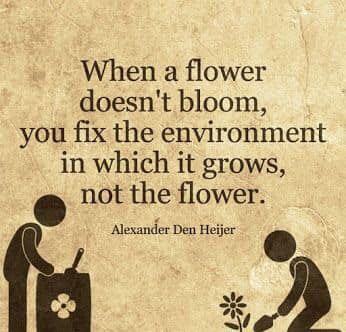
\includegraphics[width=1\linewidth,height=\textheight,keepaspectratio]{images/01-when-a-flower-doesnt-bloom.jpg}
\end{center}

\begin{center}\rule{0.5\linewidth}{0.5pt}\end{center}

\subsection{Learning objectives -
Recap}\label{learning-objectives---recap}

At the end of this session, you are now able to:

\begin{itemize}
\tightlist
\item
  \textbf{Describe} the key features of a positive learning environment,
  including the roles of verbal strategies, body language, growth
  mindset, interaction norms, perspective-taking, role modelling and
  inclusive language ✅
\item
  \textbf{Evaluate} how your behavior, language, and attitude influence
  learner motivation and engagement ✅
\item
  \textbf{Analyze} challenges affecting the learning environment during
  an Open Research training event and \textbf{evaluate} strategies to
  address them in different teaching contexts ✅
\end{itemize}

\textbf{Presenter Notes}: This where we are at now. To recap, you have
now explored the key elements of a positive learning environment and how
your communication, behavior, and attitude shape learner experiences.

You have analyzed potential challenges in Open Research and Open Science
training contexts and practiced applying strategies such as active
listening and inclusive language to support engagement and
participation.

What are your questions?

\begin{center}\rule{0.5\linewidth}{0.5pt}\end{center}

\subsection{To conclude: Survey time!}\label{to-conclude-survey-time}

ADD QR code

\begin{center}\rule{0.5\linewidth}{0.5pt}\end{center}

\subsection{To conclude: Survey time!}\label{to-conclude-survey-time-1}

\subsubsection{Question 1}

\textbf{On a scale from 1 to 5, what is your level of confidence with
actively creating a positive learning environment for your learners in
Open Research events?} (\emph{1 = not confident at all, 5 = extremely
confident, let's go})

\begin{enumerate}
\def\labelenumi{\alph{enumi}.}
\item
  1
\item
  2
\item
  3
\item
  4
\item
  5
\end{enumerate}

\subsubsection{Question 2}

\textbf{Which of the following elements of creating a positive learning
environment do you feel most confident about in your teaching at this
point?}

\begin{enumerate}
\def\labelenumi{\alph{enumi}.}
\item
  Using verbal strategies
\item
  Using non-verbal strategies
\item
  Fostering a growth mindset
\item
  Establishing norms for interaction
\item
  Using inclusive language
\item
  None of the above
\end{enumerate}

\begin{center}\rule{0.5\linewidth}{0.5pt}\end{center}

\subsection{Discussion of survey
results}\label{discussion-of-survey-results-1}

What do we see in the results?

\textbf{Presenter Notes}: Let us have a look at these results.

\textbf{Instructor Notes}: Briefly examine the answers given to each
question interactively with the group. Use visuals from the survey to
highlight specific answers.

\textbf{Accessibility Tip}: Have people work in pairs if someone did not
bring their phone/does not have a phone. This survey also cannot be
completed in an asynchronous setting.

\begin{center}\rule{0.5\linewidth}{0.5pt}\end{center}

\subsection{References}\label{references}

\protect\phantomsection\label{refs}
\begin{CSLReferences}{1}{0}
\bibitem[\citeproctext]{ref-dweckMindsetNewPsychology2006}
Dweck, C. S. (2006). \emph{Mindset: {The} new psychology of success}.
Random House Publishing Group.

\bibitem[\citeproctext]{ref-phanBridgingNeurodiversityOpen2025}
Phan, J. M., Middleton, S. L., Azevedo, F., Iley, B. J., Grose-Hodge,
M., Tyler, S. L., Kapp, S. K., Yeung, S. K., Shaw, J. J., Hartmann, H.,
\& Forrt. (2025). Bridging neurodiversity and open scholarship: {How}
shared values can guide best practices for research integrity, social
justice, and principled education. \emph{Journal of Social Issues},
\emph{81}(4), e70035. \url{https://doi.org/10.1111/josi.70035}

\bibitem[\citeproctext]{ref-rusticusWhatAreKey2023}
Rusticus, S. A., Pashootan, T., \& Mah, A. (2023). What are the key
elements of a positive learning environment? {Perspectives} from
students and faculty. \emph{Learning Environments Research},
\emph{26}(1), 161--175. \url{https://doi.org/10.1007/s10984-022-09410-4}

\end{CSLReferences}

\begin{center}\rule{0.5\linewidth}{0.5pt}\end{center}

\subsection{Additional references}\label{additional-references}

\begin{itemize}
\item
  Antosch-Bardohn, J. (2018): Nicht-intentionale Lernprozesse im Alltag
  von Studierenden. Logos Verlag.
\item
  Antosch-Bardohn, J., Beege, B., \& Primus, N. (2019). In die Lehre
  starten. UTB GmbH.
\item
  Antosch-Bardohn, J. (2019): ``Für mein Thema brennen die Studis'' -
  Lernmotivation in der Hochschullehre. In: Neues Handbuch
  Hochschullehre. Nummer 89, S. 1-18.
\item
  Hofmann, E. \& Löhle, M. (2004). Erfolgreich lernen. Hogrefe Verlag.
\item
  Kergel, D. \& Heidkamp-Kergel, B. (2020). E-Learning, EDidaktik und
  digitales Lernen. Springer VS.
\end{itemize}

\begin{center}\rule{0.5\linewidth}{0.5pt}\end{center}

\subsection{Additional resources}\label{additional-resources}

Active listening: - \url{https://www.ncbi.nlm.nih.gov/books/NBK442015/}

\begin{itemize}
\item
  \url{https://executive.berkeley.edu/thought-leadership/blog/art-active-listening}
\item
  \url{https://www.cmu.edu/student-affairs/civility/resources/active-listening.html}
\end{itemize}

\begin{center}\rule{0.5\linewidth}{0.5pt}\end{center}

\section{Thanks!}\label{thanks}

\begin{center}\rule{0.5\linewidth}{0.5pt}\end{center}

\section{Slide deck 4 from here: ACTIVATION
METHODS}\label{slide-deck-4-from-here-activation-methods}

\begin{center}\rule{0.5\linewidth}{0.5pt}\end{center}

\subsection{Interactive teaching
methods}\label{interactive-teaching-methods}

transition to activation method

\begin{center}\rule{0.5\linewidth}{0.5pt}\end{center}

\subsection{Your turn!}\label{your-turn}

Take 20 minutes in pairs to practise an activation method of your choice
in the context of a topic of your choice. Each pair demonstrates the
activity in ``class'', with the rest acting as audience.

Interactively ask participants to provide feedback on the selected
method, delivery and improvement points.

\begin{center}\rule{0.5\linewidth}{0.5pt}\end{center}

\subsection{TODO Sarah}\label{todo-sarah}

\begin{itemize}
\tightlist
\item[$\square$]
  Sort out alt text for all figures
\item[$\square$]
  Generate QR codes for teaching
\item[$\square$]
  Change CSS to include level 3 headers
\end{itemize}

\begin{center}\rule{0.5\linewidth}{0.5pt}\end{center}




\end{document}
